\chapter{Progettazione Concettuale} 

\section{Lista delle Classi}
\begin{description}
\item[PERSONA:] rappresenta una generica persona fisica all’interno del Tennis Club
\begin{itemize}
\item CodFiscale: \textit{string} \hfill 
\item Nome: \textit{string}  \hfill 
\item Cognome: \textit{string}  \hfill 
\item Sesso: \textit{enum\{“Maschio”, “Femmina”\}}  \hfill 
\item DataNasc: \textit{date}  \hfill 
\item LuogoNasc: \textit{string}  \hfill 
\item Telefono: \textit{string}  \hfill 
\item Mail: \textit{string}  \hfill 
\end{itemize}
Chiave primaria: \underline{CodFiscale} \hfill \\

Viene definita una partizione in due sottoclassi specifiche, di seguito riportate:
\item[ISTRUTTORE:] modella un istruttore, cioè una persona che tiene un corso
\begin{itemize}
\item Qualifica: \textit{string} \hfill 
\item Retribuzione: \textit{int} \hfill 
\item DataAssunzione: \textit{date} \hfill 
\end{itemize}
\item[SOCIO:] modella un socio, cioè una persona non istruttore, che frequenta il Tennis Club ValleVerde
\begin{itemize}
\item DataIscrizione: \textit{date} \hfill 
\item Livello: \textit{enum\{'Principiante', 'Intermedio', 'Esperto'\}} \hfill 
\end{itemize}
\item[ACCOUNT:] modella un account posseduto da una persona del Tennis Club
\begin{itemize}
\item UserName: \textit{string} \hfill 
\item Admin: \textit{bool} \hfill 
\item Hash: \textit{string} \hfill 
\end{itemize}
Chiave primaria (definita come identificatore esterno): \underline{CodFiscale} \hfill 
\item[CORSO:] modella un generico corso tenuto all’interno della scuola Tennis del Tennis Club
\begin{itemize}
\item CodCorso: \textit{int} \hfill
\item NomeCorso: \textit{string} \hfill
\item TipoCorso: \textit{enum\{‘Principiante’,’Intermedio’,’Avanzato’\}} \hfill
\item Attivo: \textit{bool} \hfill
\end{itemize}
Chiave primaria: \underline{CodCorso} \hfill 
\item[LEZIONE:] rappresenta una lezione di un corso
\begin{itemize}
\item CodLezione: \textit{int} \hfill 
\end{itemize}
Chiave primaria: \underline{(CodCorso,CodLezione)} \hfill 
\item[CAMPO:] modella un campo da Tennis
\begin{itemize}
\item CodCampo: \textit{tinyint} \hfill 
\item TipoSup: \textit{enum\{‘Terra rossa’, ‘Erba sintetica’, ‘Playit’\}}
\end{itemize}
Chiave primaria: \underline{CodCampo} \hfill 
\item[PRENOTAZIONE:] modella una prenotazione di un campo
\begin{itemize}
\item Data: \textit{date} \hfill 
\item Ora: \textit{int} \hfill  
\end{itemize}
Chiave primaria: \underline{(CodCampo,Data,Ora)} \hfill 
\end{description}

\section{Lista delle Associazioni}

\begin{itemize}
\item \textsc{Persona - Account:} \textbf{Possiede}
\begin{itemize}
\item Ogni persona possiede un solo account. Ogni account è posseduto da una sola persona.
\item Molteplicità 1:1
\item Totalità: Totale in entrambi i sensi.
\end{itemize}

\item \textsc{Persona – Prenotazione:} \textbf{Fa}
\begin{itemize}
\item Una persona fa zero o più prenotazioni, ogni prenotazione viene fatta da una sola persona.
\item Molteplicità: 1:N
\item Totalità: Totale da Prenotazione verso Persona, parziale da Persona verso Prenotazione.
\end{itemize}

\item \textsc{Istruttore – Corso:} \textbf{Tiene}
\begin{itemize}
\item Un istruttore tiene zero o più corsi, ogni corso è tenuto da un solo istruttore.
\item Molteplicità: 1:N
\item Totalità: Parziale ambo i lati
\end{itemize}
\item \textsc{Socio - Corso:} \textbf{IscrittoCorso}
\begin{itemize}
\item Un socio è iscritto a zero o più corsi, un corso ha zero o più soci iscritti
\item Molteplicità: N:M
\item Totalità: Parziale ambo i lati
\end{itemize}
\item \textsc{Corso - Lezione:} \textbf{CompostoDa}
\begin{itemize}
\item Un corso è composto da zero o più lezioni, zero o più lezioni compongono un corso.
\item Molteplicità: 1:N
\item Totalità: Parziale da Corso a Lezione, totale da Lezione a Corso
\end{itemize}
\item \textsc{Prenotazione - Campo:} \textbf{Riguarda}
\begin{itemize}
\item Una prenotazione riguarda un campo, ogni campo ha zero o più prenotazioni.
\item Molteplicità: 1:1
\item Totalità: Totale da Prenotazione a Campo, parziale da Campo a Prenotazione 
\end{itemize}
\item \textsc{Prenotazione – Lezione:} \textbf{Crea}
\begin{itemize}
\item Una prenotazione crea zero o una lezione, una lezione viene creata da una prenotazione.
\item Molteplicità: 1:1
\item Totalità: Parziale da Prenotazione a Lezione, Totale da Lezione a Prenotazione
\end{itemize}
\end{itemize}

\section{Descrizione della Gerarchia}
L'unica gerarchia presente nello schema concettuale riguarda la superclasse \textit{Persona} che si divide nelle due sottoclassi specializzate \textit{Istruttore} e \textit{Socio}.\\

Tale generalizzazione è \textit{Totale} in quanto ogni occorrenza di \textit{Persona} è anche occorrenza di \textit{Istruttore} o di \textit{Socio} (ricordiamo che \textit{Persona} modella una persona fisica all'interno del Tennis Club).\\
La generalizzazione è inoltre \textit{esclusiva}, in quanto una \textit{Persona} rappresentata dalla superclasse non può essere contemporaneamente \textit{Socio} e \textit{Istruttore}.\\

Le due sottoclassi specializzate prevedono degli attributi propri per modellare gli istruttori (\textit{Qualifica}, \textit{Retribuzione} e \textit{DataAssunzione}) e i soci (\textit{DataIscrizione} e \textit{Livello}).

\section{Vincoli di Integrità aggiuntivi}

\begin{itemize}
\item La retribuzione di un istruttore non puo' essere un valore negativo (minore od uguale a zero).
\item La retribuzione di un istruttore non puo' essere inferiore alla retribuzione base, fissata ad 800 \euro .
\end{itemize}

\section{Schema concettuale E-R}
\begin{figure}[H]
 \centering
  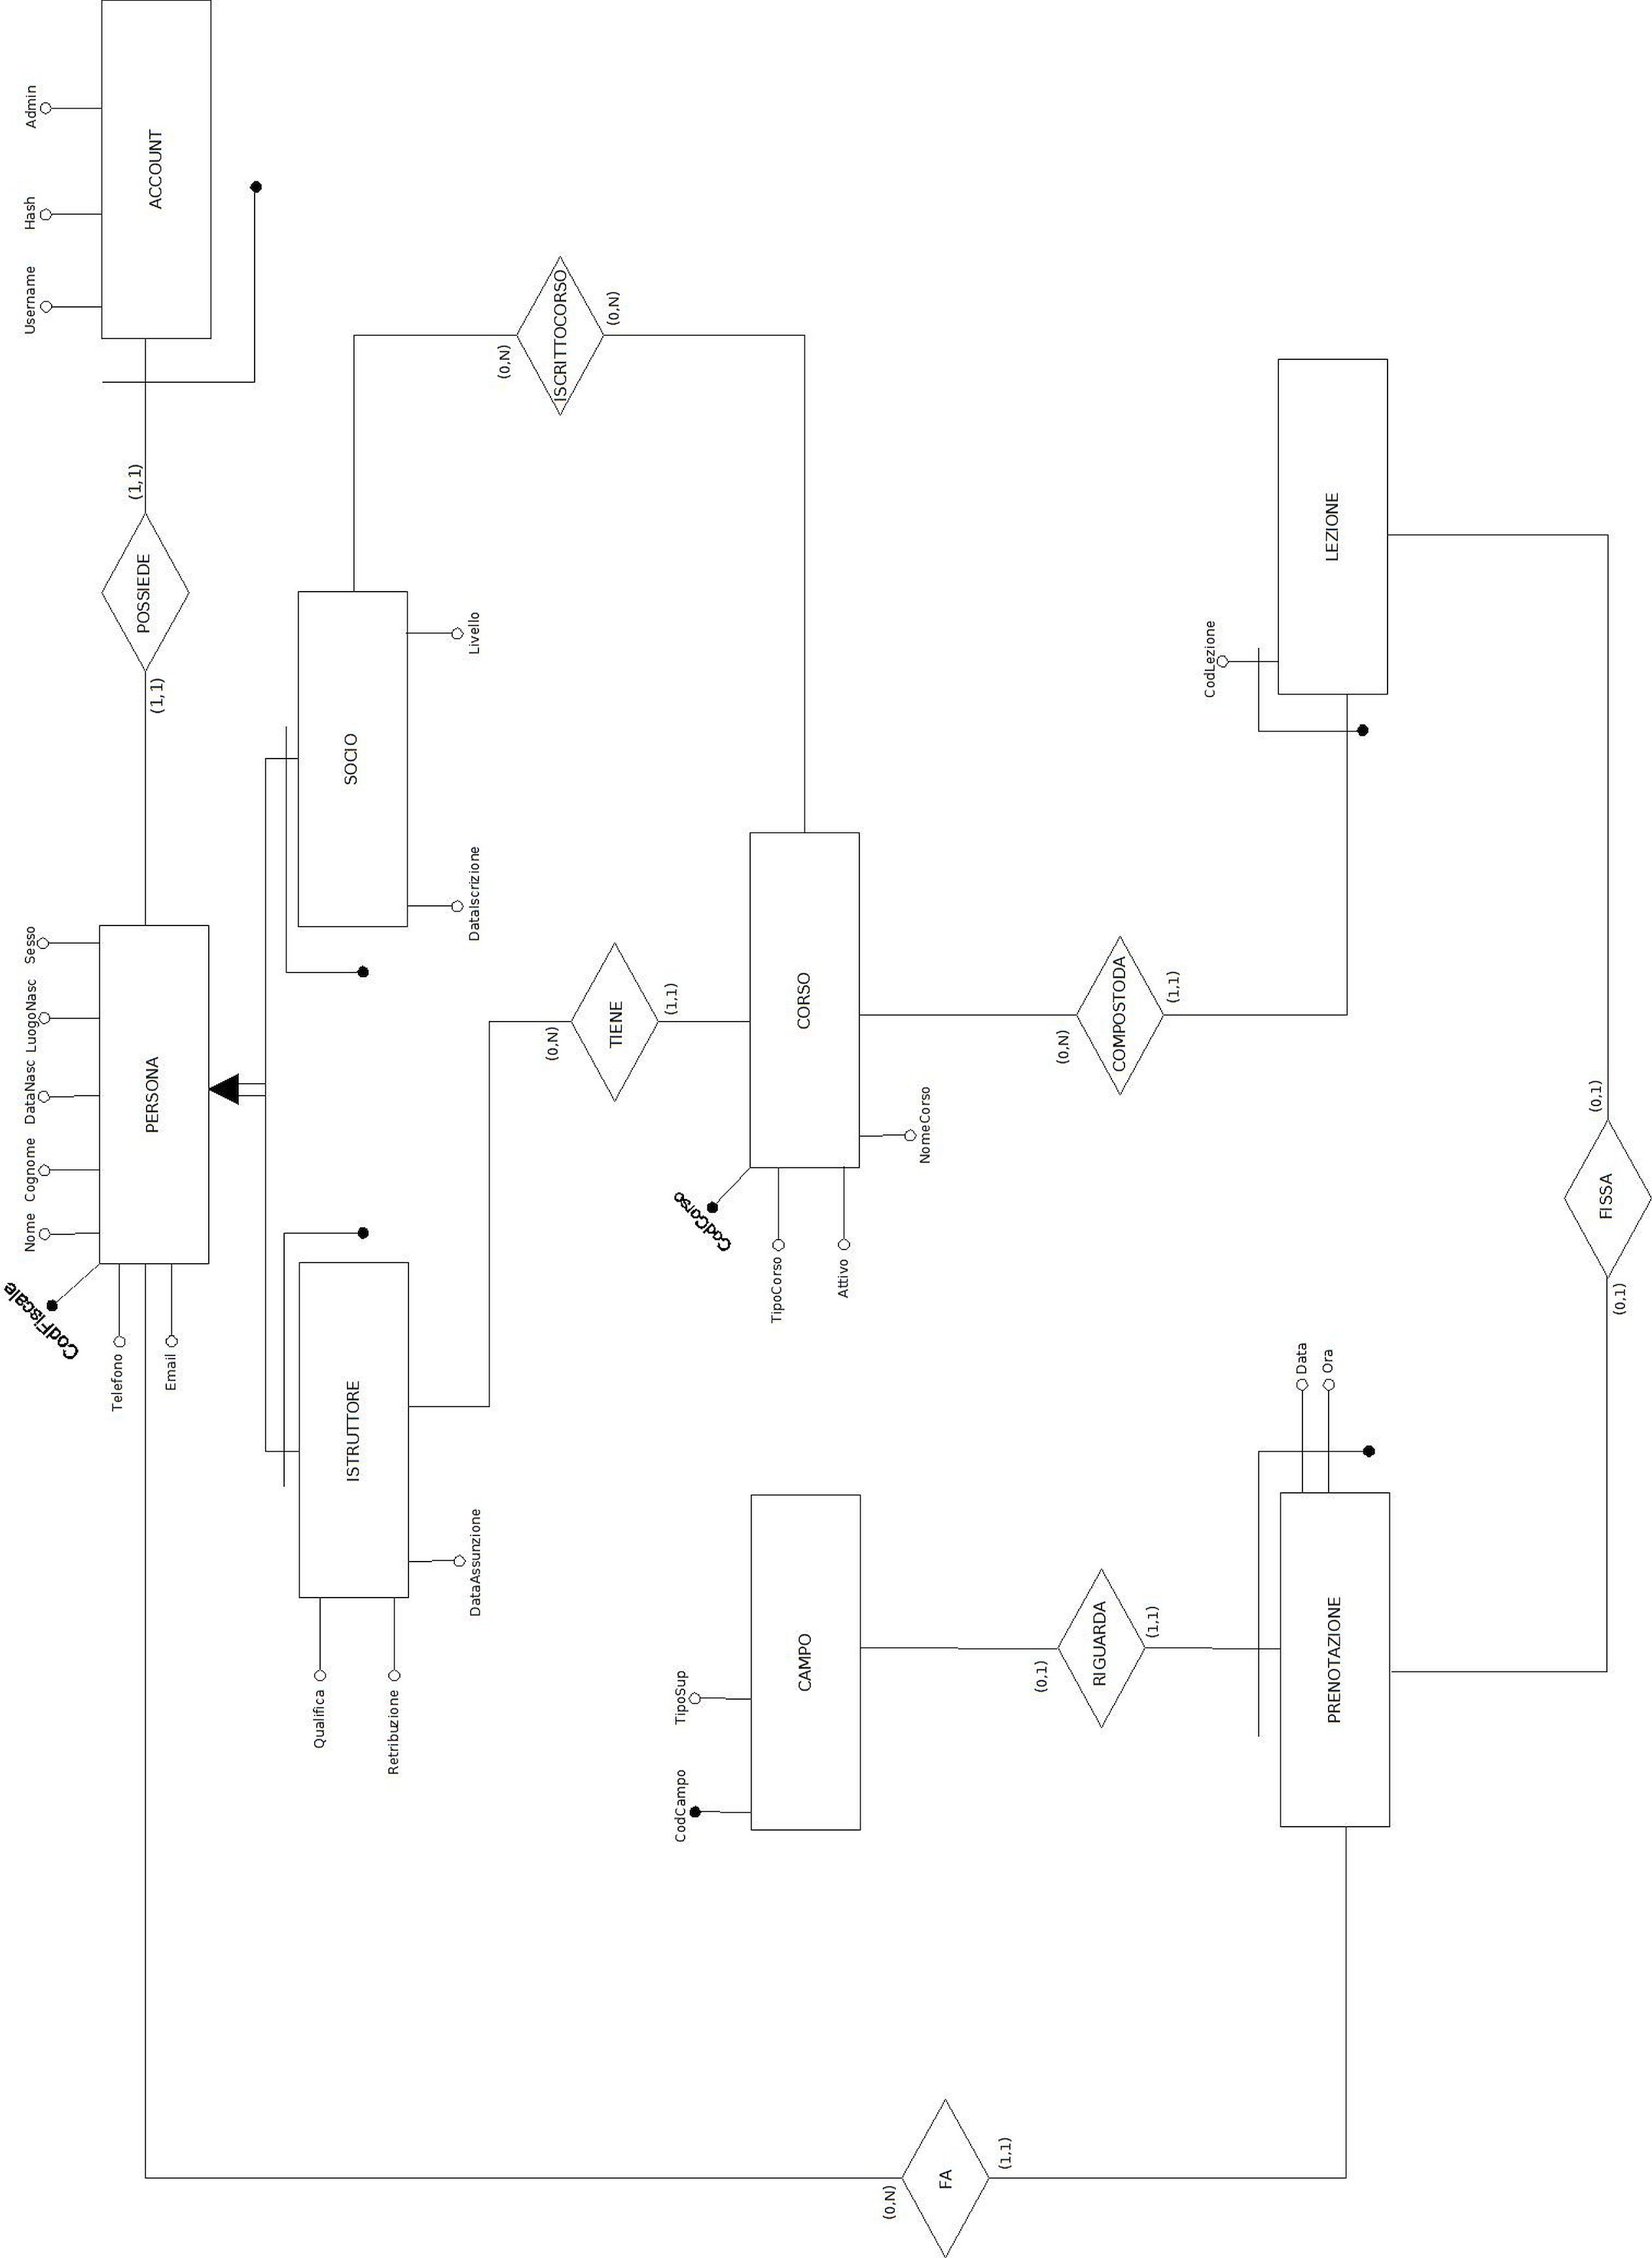
\includegraphics[width=\textwidth, height=\textheight]{images/ER_FINALE.jpg}
\caption{Schema Concettuale E-R}
\end{figure}